\begin{figure}[!]
    \centering
    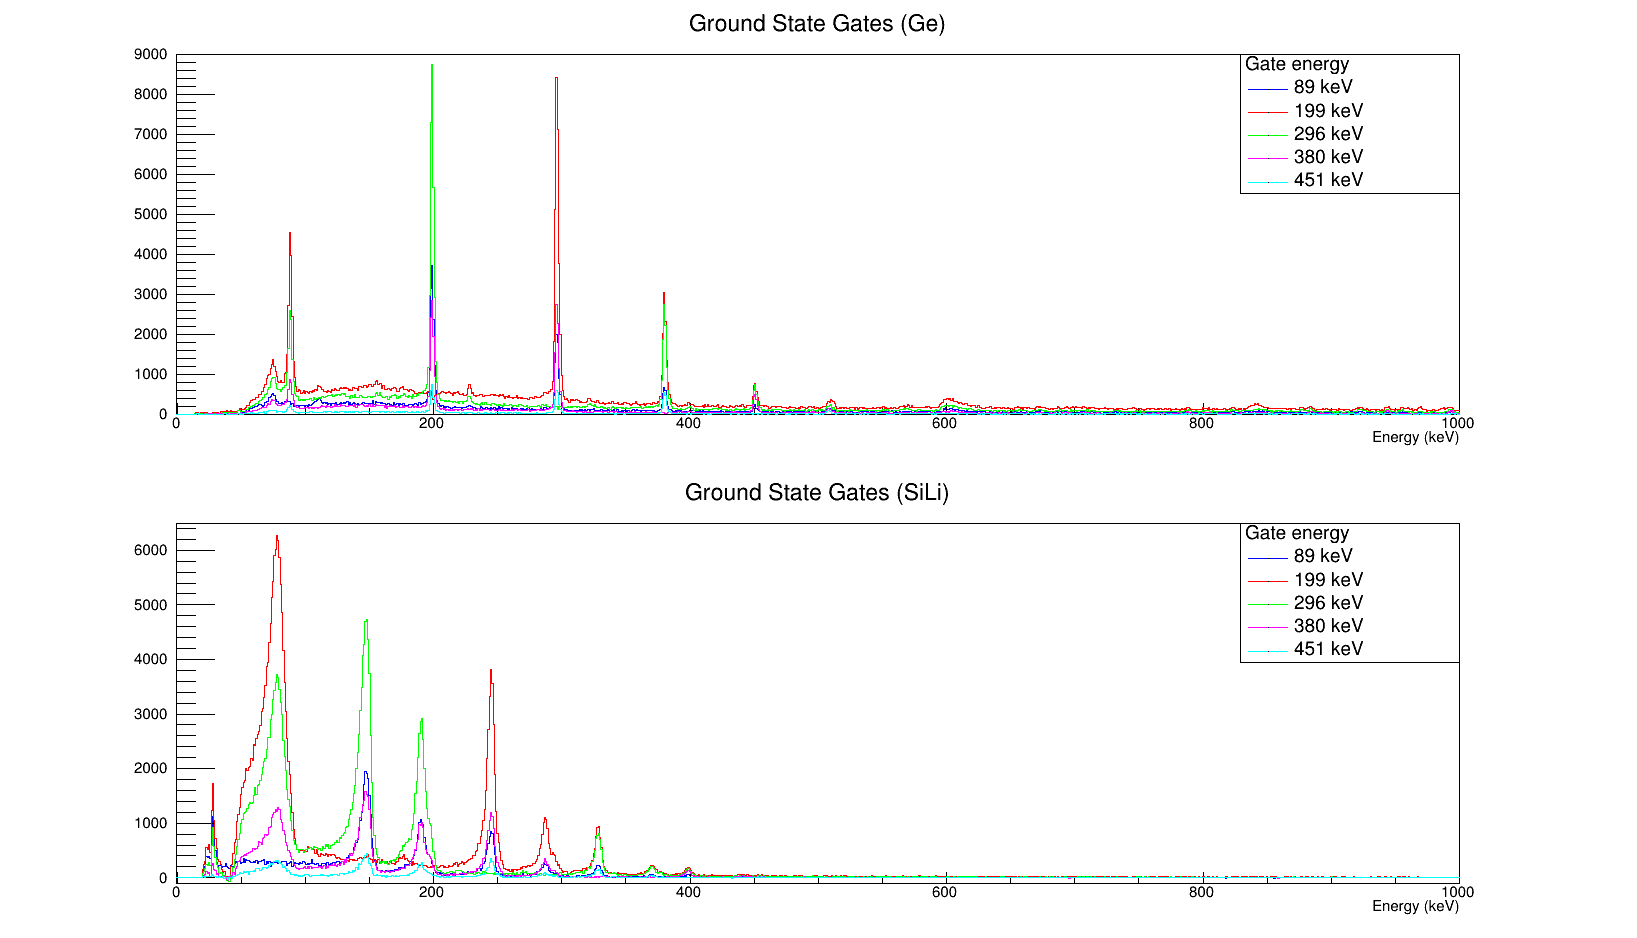
\includegraphics[scale=0.27]{156GdTablesAndFigs/156GS_stack.png}
    \caption{Spectra gated on the ground state band lines of $^{156}$Gd. As can be seen, some lines do not appear in different gates. Comparison of these gates, for instance 199 keV ($4^+\rightarrow2^+$) and 296 keV ($6^+\rightarrow4^+$), yields a list of transitions that directly populate the interim level (in the example, the $4^+$ state). The 89 keV line, although the lowest transition in the ground state band, has a low yield due to efficiency, and is reflected in the relative size of the peaks. The 199 keV peak in the gamma spectrum is much larger from the 296 keV transition than the 89 keV transition.}
    \label{fig:156_GS_Gate}
\end{figure}